\section{The LHC and the CMS detector} \label{section: CMS}

% Add LHC

The Large Hadron Collider (LHC) is currently the largest and highest-energy particle accelerator. It is a 27-km long circular hadron accelerator located 100 meters underground at CERN, near Geneva, on the border between France and Switzerland. Protons are accelerated and collide every 25 ns at the four interaction points, corresponding to the four main experiments: ATLAS \cite{ATLAS}, CMS \cite{CMS}, LHCb \cite{LHCb}, and ALICE \cite{ALICE}. Figure \ref{fig: LHC} shows the  LHC complex as well as the location of the four main experiences.

\begin{figure}[hbt]
    \centering
    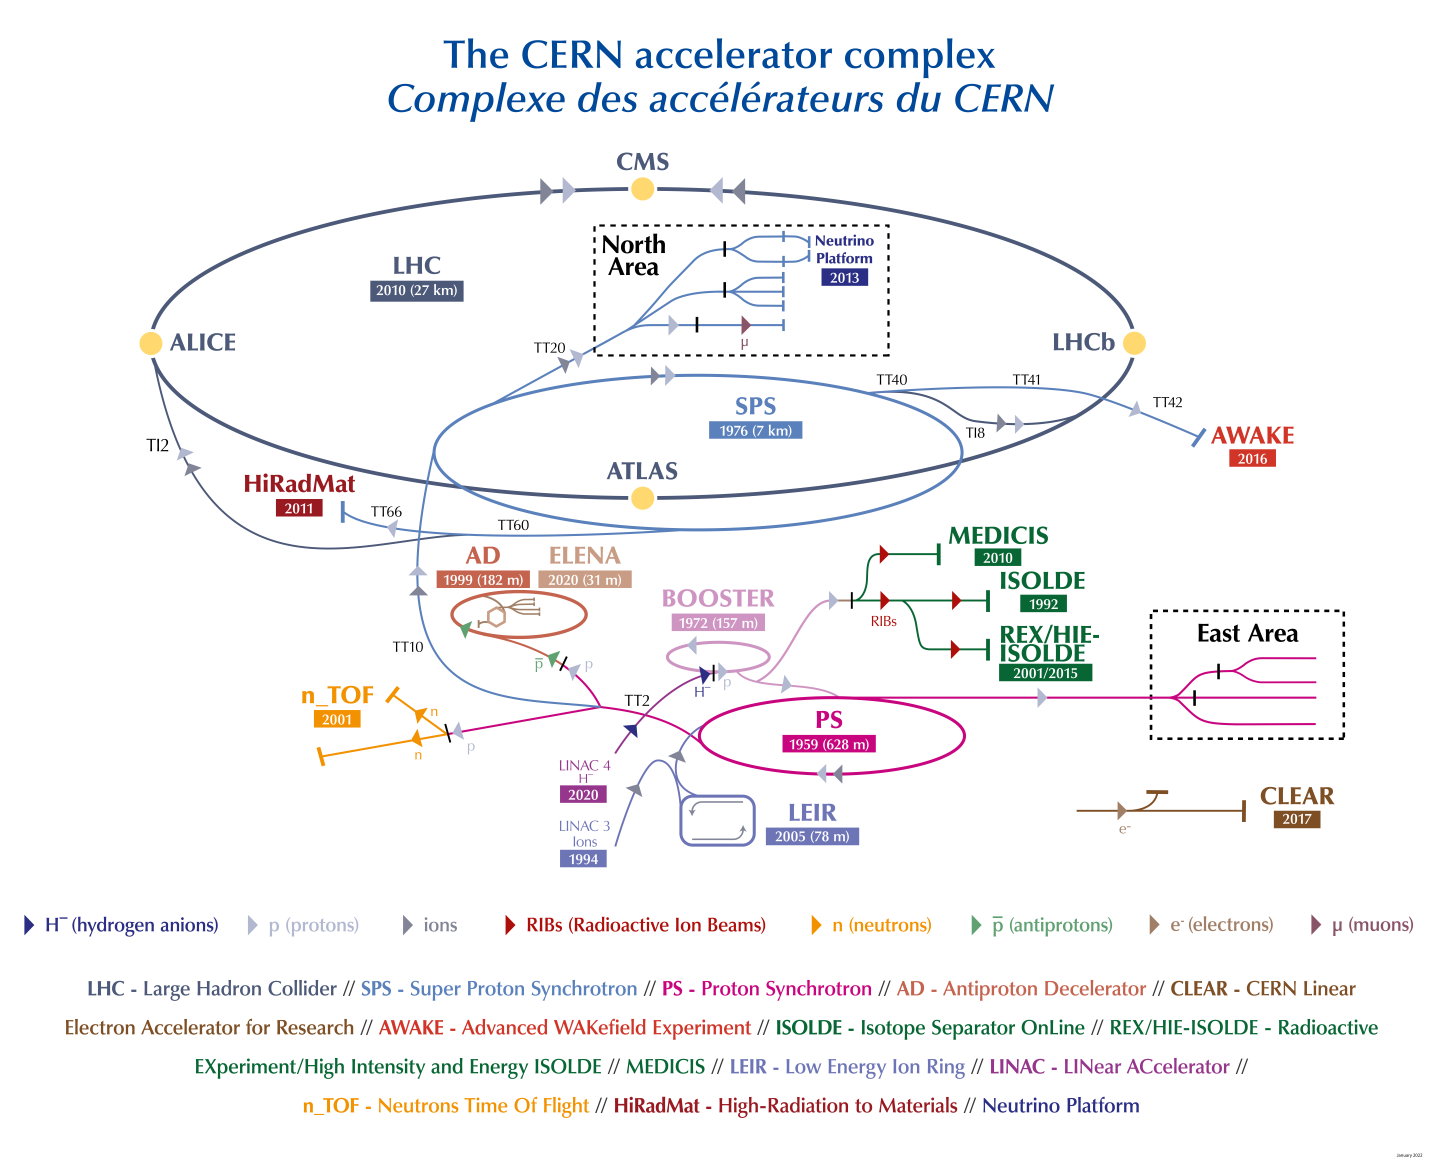
\includegraphics[width=0.7\linewidth]{Images/3.CMS/CCC-v2022.png}
    \caption{The Large Hadron Collider (LHC) complex \cite{LHCFIG}.}
    \label{fig: LHC}
\end{figure}

Ever since the LHC started taking data, there have been 3 periods of data taking each one referred to as "Run". Figure \ref{fig: Runs} shows the integrated luminosity of the three periods of data taking (Run 1, 2, and 3) as well as the center of mass energy of the collisions $\sqrt{s}$ in each period. The integrated luminosity \lumi is the integral of the luminosity with respect to time:

\begin{equation}
    \lumi= \int \frac{1}{\sigma} \frac{dN}{dt} dt
\end{equation}

\noindent where $\sigma$ is the cross-section and $N$ the number of events detected.

\begin{figure}[hbt]
    \centering
    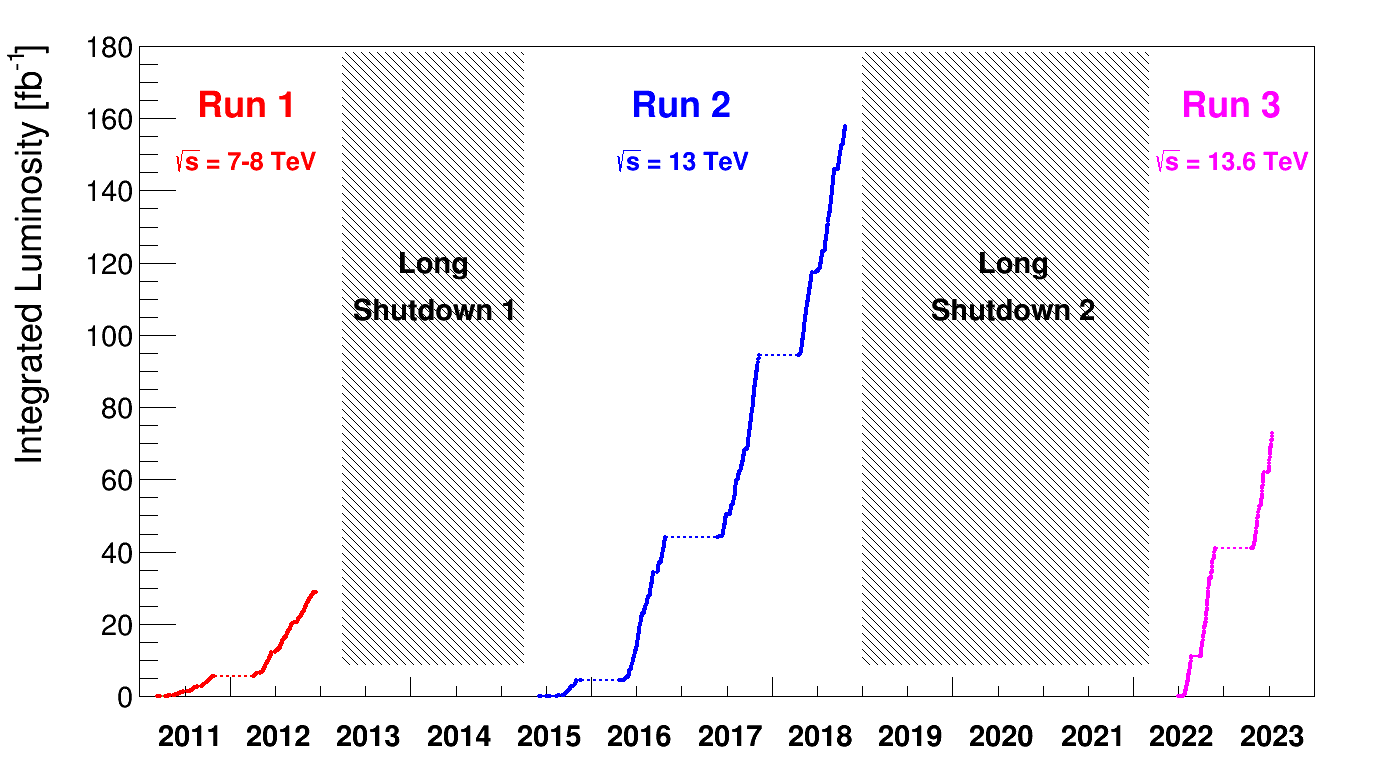
\includegraphics[width=0.5\linewidth]{Images/3.CMS/Run plots.png}
    \caption{Integrated luminosity delivered by LHC as a function of data-taking years. The center of mass energy of the collisions $\sqrt{s}$ is also reported \cite{Runplot}.}
    \label{fig: Runs}
\end{figure}

%https://be-dep-op-lhc.web.cern.ch

%explain run 2 and 3

CMS (Compact Muon Solenoid) is one of the four detectors of the LHC. It is made of (starting from the center) a tracker, made of silicon sensors, that can measure the trajectory of the particles. Then, to measure the energy of the electrons and the photons, the electromagnetic calorimeter (ECAL) is used. The latter stops these particles completely via interactions (showers) with the PbWO$_4$ crystals. ECAL is surrounded by HCAL, the hadron calorimeter, which stops the hadrons and reconstructs their energy. This is followed by a large superconducting magnet, inducing a very strong magnetic field (3.81 T), that bends the trajectory of the particles. This allows to retrieve information in the tracker about the momentum and the sign of the charge of the particle due to the bending of its trajectory by the magnetic field. The last layer of the detector is the muon detector. Figure \ref{fig: CMS detector} shows the different layers of the CMS detector. 

\begin{figure}[hbt]
    \centering
    \includegraphics[width=0.8\linewidth]{Images/3.CMS/cms_160312_02.png}
    \caption{A three-dimensional view showing the different layers of the CMS detector \cite{CMS3D}.}
    \label{fig: CMS detector}
\end{figure}

Collisions in the detector take place every 25 ns, to retrieve the information from the collisions, CMS uses a multi-level trigger system. The CMS trigger system consists of:
\begin{itemize}
    \item Level 1 (L1) trigger: this trigger is implemented using FPGAs (Field Programmable Gate Array) and ASICs (Application-Specific Integrated Circuit) and allows for a fast readout of the detector with limited granularity. \cite{L1Trigger}, \cite{Trigger}
    \item High Level Trigger (HLT): the events that are accepted by the L1 trigger are passed to the HLT. This trigger is implemented as software algorithms that run on large clusters of commercial processors. \cite{HLT}, \cite{Trigger}
\end{itemize}

Figure \ref{fig: coord syst} shows the 3D coordinate system of the CMS detector. The accelerated proton beams are along the $z$-axis and the collisions occur at the interaction point (IP). The $xy$-plane as is observed in Figure \ref{fig: coord syst} is the transverse plane.

\begin{figure}[hbt]
    \centering
    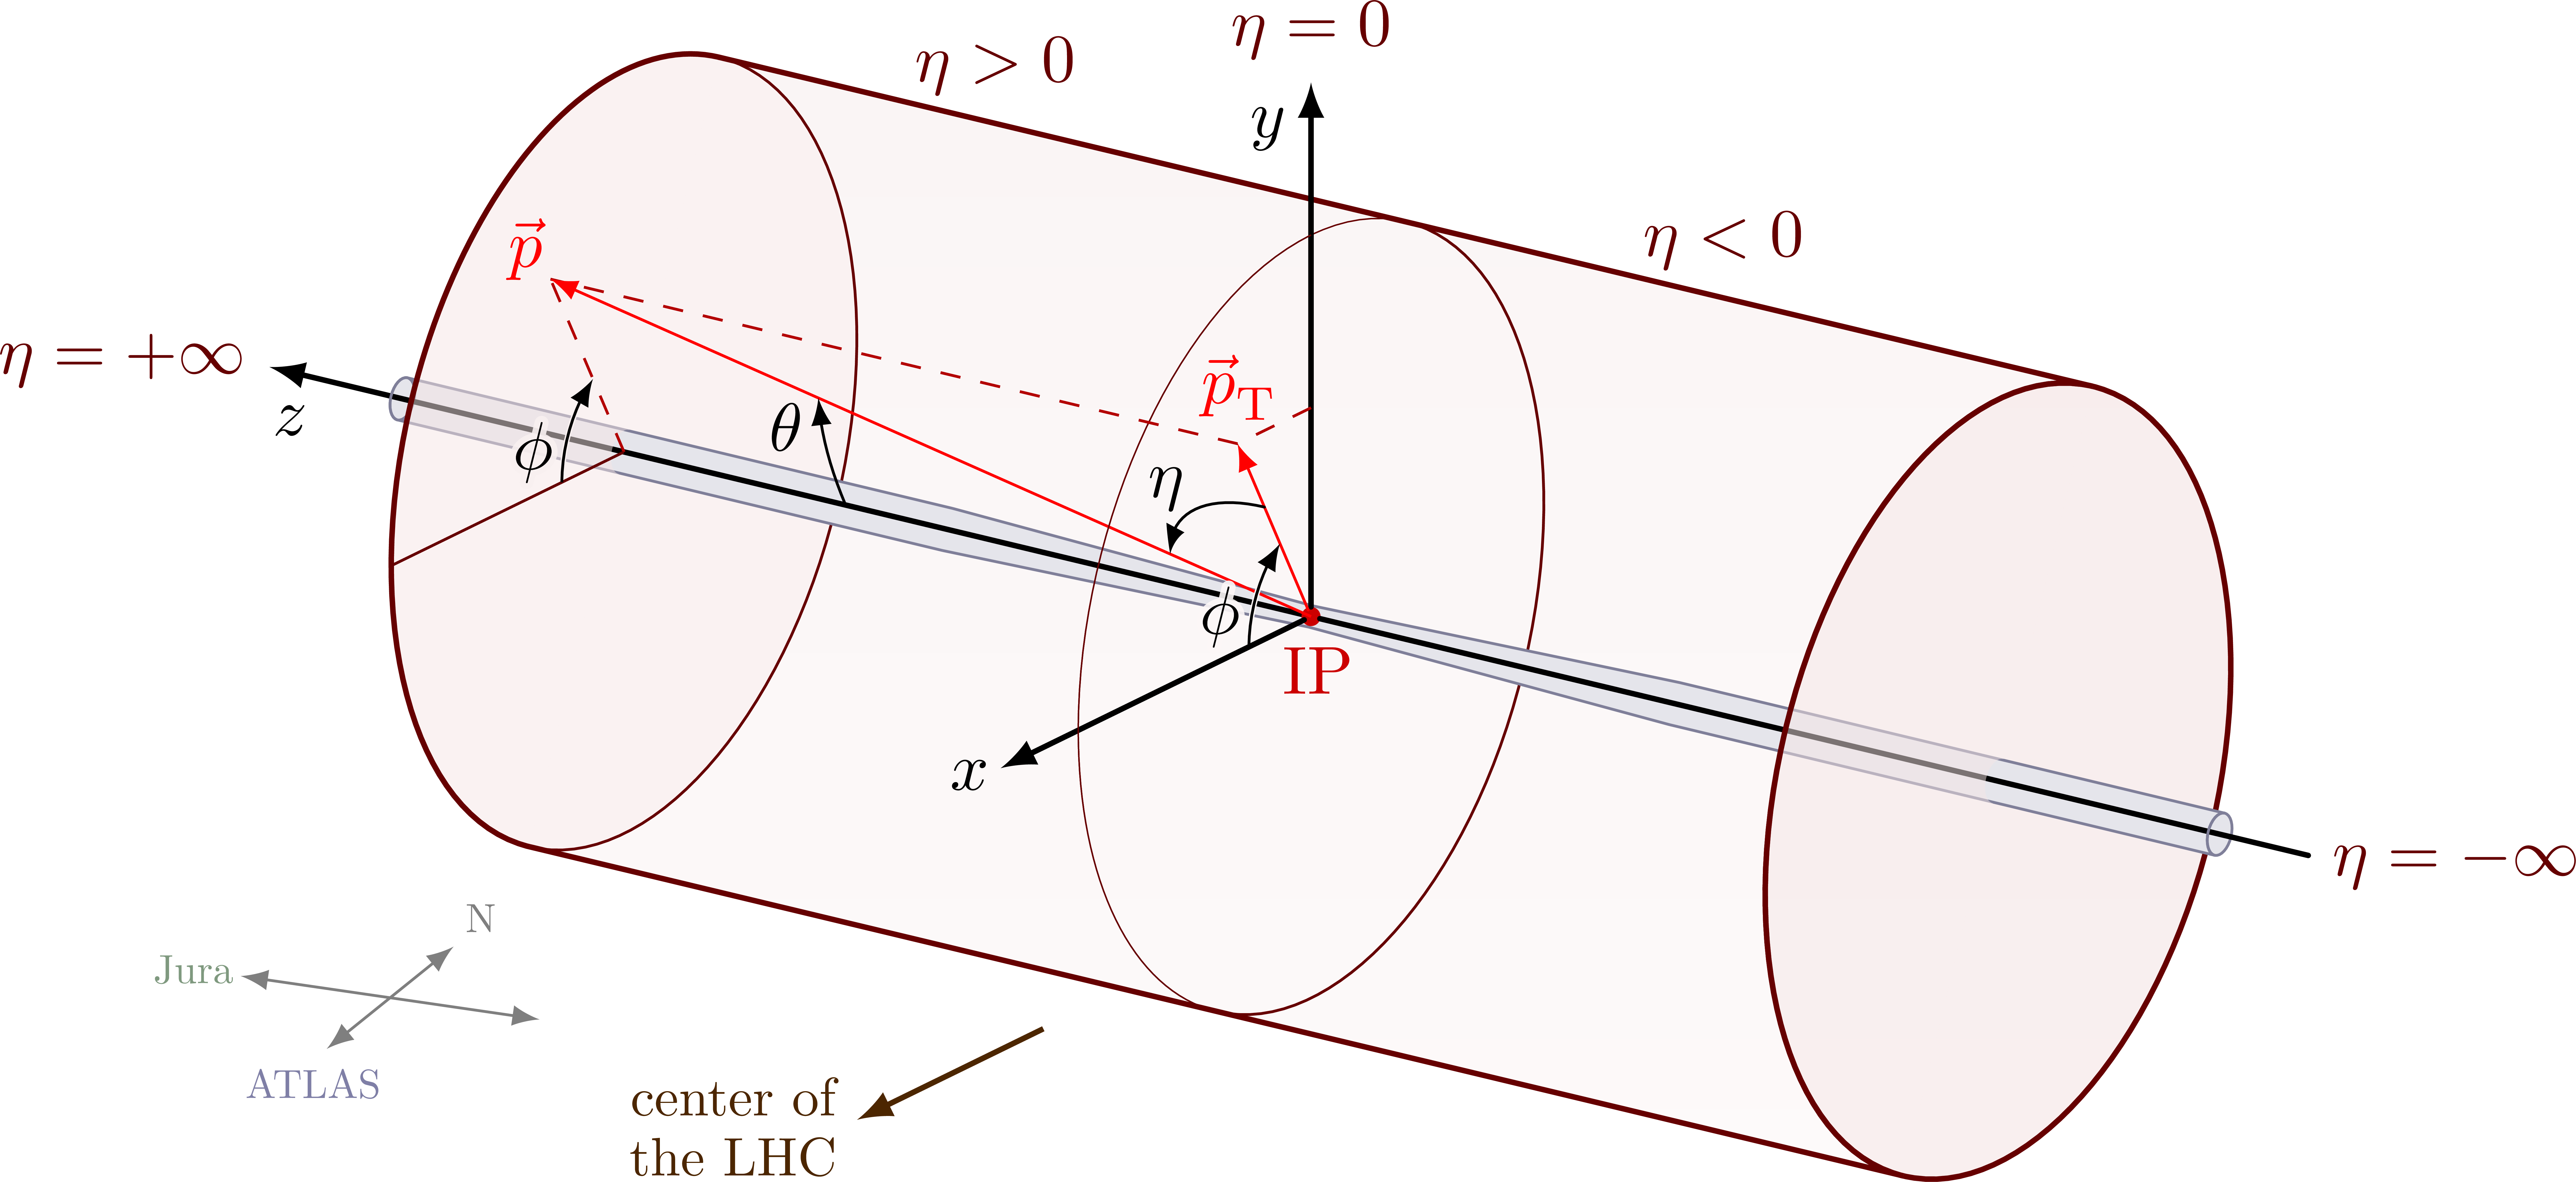
\includegraphics[width=0.7\linewidth]{Images/4.HH4b Analysis/axis3D_CMS-005.png}
    \caption{Coordinate system of the CMS detector \cite{CMScoord}.}
    \label{fig: coord syst}
\end{figure}

\subsection{Kinematic variables used in the HH $\to$ 4b analysis} \label{subsection: kinematic vars}
The definitions of the observables that will be used in the following Sections are reported in this Section. Figure \ref{fig: coord syst} shows the CMS coordinate system.

\begin{itemize}
    \item The pseudorapidity $\eta$, defined as:
    \begin{equation}
        \eta=-\mathrm{ln}\bigg(\text{tan}(\frac{\theta}{2})\bigg)
    \end{equation}
    with $\theta$ being the angle between the beam axis ($z$) and the deviated particle or jet. When the deviation is low, the pseudo-rapidity either tends to $\pm \infty$ depending on whether it is along the $z$-axis or in the opposite direction (see Figure \ref{fig: coord syst}).
    \item $\Phi$ is the azimuthal angle in the $xy$ plane. Since this angle is in the transverse plane it is Lorentz-invariant.
\end{itemize}

Since the physics processes should not depend on the reference frame, the $\eta, \Phi$ is the metric used in the detector since $\Delta \eta$ and $\Phi$ is Lorentz-invariant. 

\begin{itemize}
    \item Transverse momentum of the particles \pt: projection of the momentum in the transverse plane, as shown Figure \ref{fig: coord syst}. In proton-proton collisions, the colliding partons carry a fraction of z-momentum that depends on the parton distribution functions (PDF), leading to a boost of the particles. To avoid this, the transverse momentum is used. 
    \item $\Delta R$ is the angular distance between two objects, for instance, jets. It is defined as:
    \begin{equation}
        \Delta R = \sqrt{(\Delta \eta)^2 + (\Delta \Phi)^2 }
    \end{equation}
    \item \Ht is the sum of all the \pt of the jets in a given reconstructed event.
    \item b-tagging is the identification (tagging) of jets containing the decay of a B hadron (b jets). The ParticleNet tagger (PNet), initially introduced in \cite{PNet},
    is used to identify the flavor of the jet (b-, c-, light-flavour jets or gluon jets). Thus, this network provides a score (b-tag score) which is correlated to the probability of a jet to originate from a b-quark, a c-quark or a light-flavor quark. The closer the score is to one, the more likely it is to be a jet originating from a b quark. Three working points (WPs) are defined:
    \begin{itemize}
        \item Tight WP: 0.1\% of misidentification (mistagging) of the flavor of the jet, i.e. only 0.1\% of the events above this point are jets coming from a quark with a lighter flavor or a gluon but are classified as b jets.
        \item Medium WP: 1\% of misidentification of the flavour of the jet
        \item Loose WP: 10\% of misidentification of the flavor of the jet
    \end{itemize}
    \item \pt regressed (\pt reg): by using the ParticleNet neural network it is possible to correct the raw jet \pt to the generator-level jet energy. To do so, two components are taken into account: the \pt is adjusted to be closer to the generator-level jet \pt, and the presence of neutrinos, not reconstructed in the detector, is also taken into account, by summing their transverse momentum to the jet.
    \item Impact parameter $d_0$ is the distance of closest approach between the daughter particle trajectory and the mother particle production point. The impact parameter (IP) is shown in Figure \ref{fig: IP}. The impact parameter in the $xy$ plane is noted $d_{xy}$ and along the z-axis $d_z$.
\end{itemize}

\begin{figure}[hbt]
    \centering
    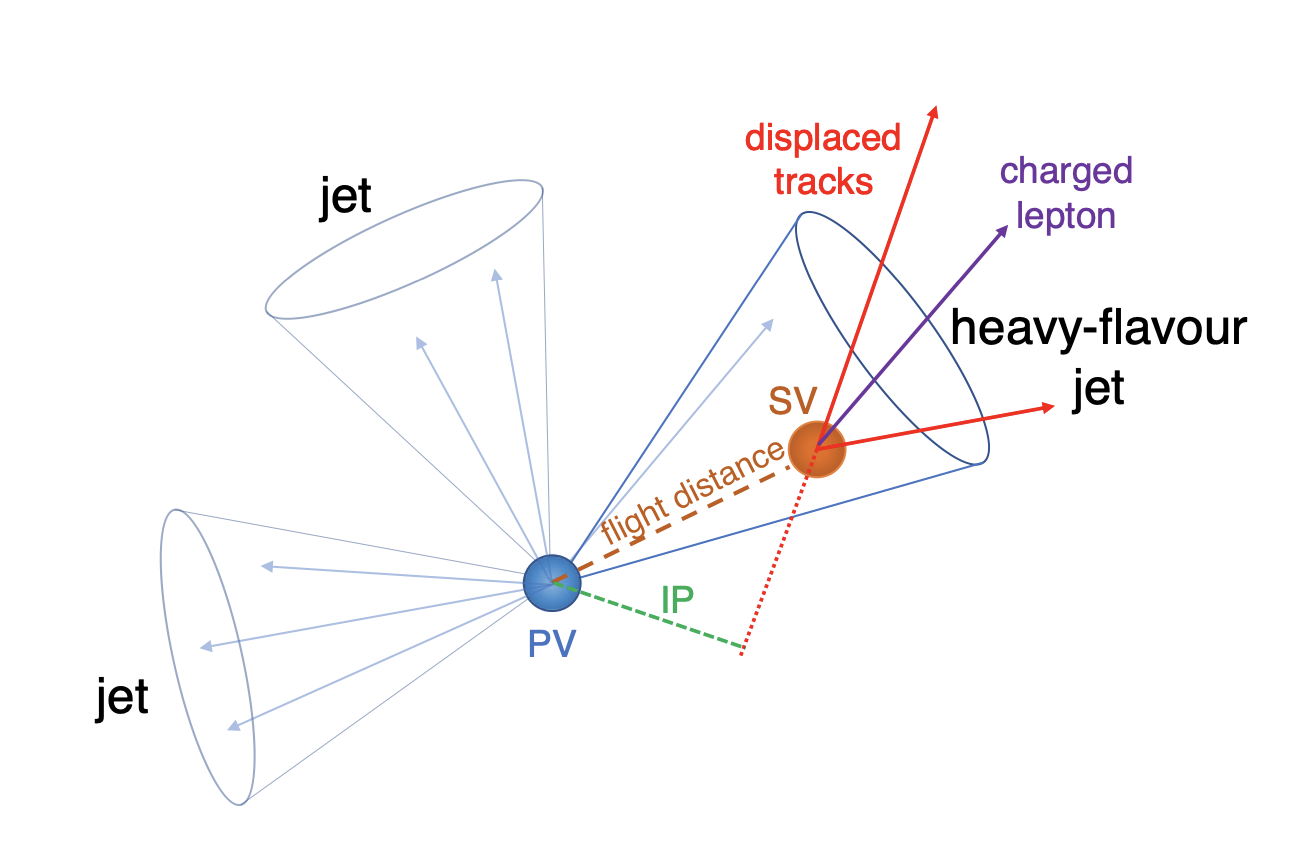
\includegraphics[width=0.5\linewidth]{Images/3.CMS/impact parameter.png}
    \caption{Sketch showing the definition of the impact parameter (IP) as well as primary (PV) and secondary (SV) vertices in heavy-flavor jet production \cite{IP}. }
    \label{fig: IP}
\end{figure}


%Maybe nno need of too much on this part

% \subsection{Tracker}
% \subsection{Electromagnetic calorimeter (ECAL)}
% \subsection{Hadronic Calorimeter (HCAL)}
% \subsection{Solenoid}
% \subsection{Muon detector}
% \subsection{Triggers}
% \subsection{Event recontsruction}
% \subsubsection{Primary Vertex}
% \subsubsection{Pile-up}
% \subsubsection{Jet reconstruction}
% \subsubsection{Missing Energy}
% \subsubsection{B-tagging} \label{Btagging} b tag algorithms are used and the fact that we use th e btag fpr the morphing to 2b to 4b
% \subsubsection{pt reg} \label{subsubsec: btag-ptreg}
% The \pt regressed is the one computed using a DNN. The main idea is that, we train a DNN with information from the reco jets and we try to retrieve the original energy if these jets. For efficiency purposes this DNNN gives out the ratio of the predicted E/ original E. To improve the analysis, we use \pt reg, which means that we multiply the \pt measured by the detector times this ratio, which allows us ti have a more precise value of thee \pt of the objects we are using.
% \subsection{Monte-Carlo}
% \subsubsection{Gen/Reco jets}

% 0.1 perccent if misidentification if the flaviur
% 1
% 10